---
id: tkz-euclide-ejemplo-63
title: "Circunferencia y ángulos"
description: "Creación de una circunferencia y ángulos"
keywords: [circunferencia, angulo,taller4]
tags: [tkzDrawCircle,tkzFillAngle,tkzFillAngle,tkzLabelAngle]
sort: 63
---
\documentclass[tikz,border=2mm]{standalone}
\usepackage{tkz-base}
\usepackage{tkz-euclide}

\begin{document}
    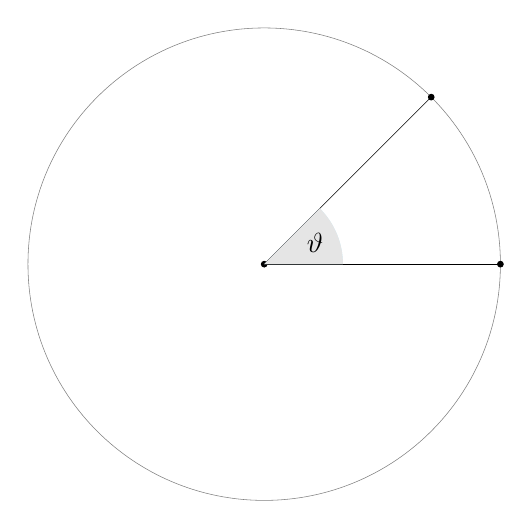
\begin{tikzpicture}
        % Paso 1: Define puntos de un radio.
        \tkzDefPoint(18,5){U} % punto central
        \tkzDefPoint(21,5){V} % punto de circunferencia

        % Paso 2: Dibuja la circunferencia
        \tkzDrawCircle(U,V)
        
        % Paso 3: Define punto W en la circunferencia
        % a 45 grados del punto V
        \tkzDefPointOnCircle[through=center U angle 45 point V]
            \tkzGetPoint{W}

        % Paso 4: Dibuja los puntos del centro y circunferencia
        \tkzDrawPoints(U,V,W)

        % Paso 5: dibuja segmentos del sector circular 
        % y deja en evidencia el ângulo WUV
        \tkzDrawSegments(W,U U,V)
        
        % Paso 6: Rellena ángulo de color cyan con opacidad 20%
        \tkzFillAngle[cyan!20](V,U,W) % ∠VUW
        
        % Paso 7: Marca y etiqueta el ángulo
        \tkzFillAngle(V,U,W) % ∠VUW
        \tkzLabelAngle[pos=0.7](V,U,W){$\vartheta$} % ∠VUW
    \end{tikzpicture}
\end{document}